% fig_zone2_diff_by_state.tex
% Bar chart: Zone 2 differential (3ph BB2 fault) across GOOSE states
% Shows reduction from S1_STALE → S1a_GEN_OK → S2_BOTH_OK
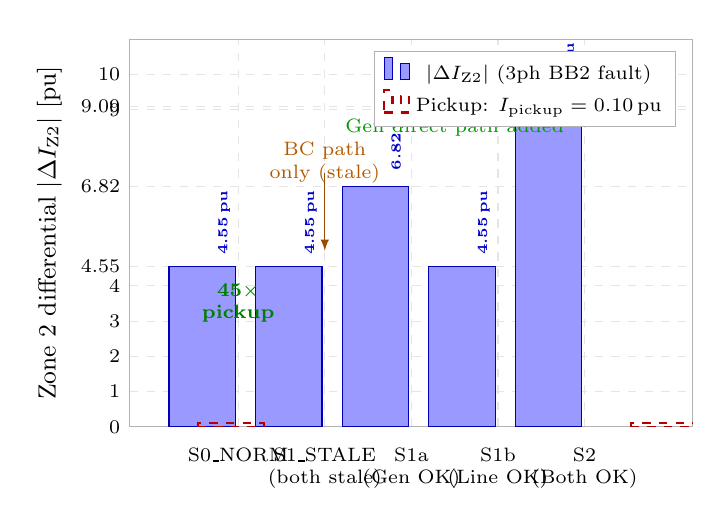
\begin{tikzpicture}
\begin{axis}[
  name        = z2ax,
  ybar,
  bar width   = 24pt,
  width       = 0.72\textwidth,
  height      = 6.5cm,
  ylabel      = {Zone 2 differential $|\Delta I_{\rm Z2}|$ [pu]},
  ylabel style= {font=\small},
  ymin=0, ymax=11,
  ytick       = {0,1,2,3,4,4.545,6.818,9,9.091,10},
  yticklabels = {0,1,2,3,4,4.55,6.82,9,9.09,10},
  yticklabel style={font=\scriptsize},
  xtick       = {1,2,3,4,5},
  xticklabels = {
    {S0\_NORM},
    {S1\_STALE\\(both stale)},
    {S1a\\(Gen OK)},
    {S1b\\(Line OK)},
    {S2\\(Both OK)}
  },
  xticklabel style={font=\scriptsize, align=center},
  enlarge x limits=0.15,
  legend style={at={(0.97,0.97)}, anchor=north east,
                font=\scriptsize, draw=gray!60},
  grid         = major,
  grid style   = {gray!20, dashed},
  tick style   = {draw=none},
  axis line style={gray!60},
]

% Zone 2 differential values (3ph BB2 fault):
% S0_NORM:   I_Gen_via_BC = V/(Z_SRC+Z_BC)*0.5 ... wait, S0 uses I_Gen via BC directly
% Actually from study output:
% S0_NORM: 4.545, S1_STALE: 4.545, S1a: 6.818, S1b: 4.545, S2: 9.091

\addplot[fill=blue!40, draw=blue!70!black]
  coordinates {(1,4.545) (2,4.545) (3,6.818) (4,4.545) (5,9.091)};
\addlegendentry{$|\Delta I_{\rm Z2}|$ (3ph BB2 fault)}

% Pickup threshold line
\addplot[red!70!black, thick, dashed, mark=none, domain=0.5:5.5, samples=2]
  ({x}, {0.10});
\addlegendentry{Pickup: $I_{\rm pickup}=0.10$\,pu}

% ---- Value annotations ----------------------------------------
\node[font=\tiny\bfseries, blue!80!black, rotate=90]
  at (axis cs:0.84, 5.8) {4.55\,pu};
\node[font=\tiny\bfseries, blue!80!black, rotate=90]
  at (axis cs:1.84, 5.8) {4.55\,pu};
\node[font=\tiny\bfseries, blue!80!black, rotate=90]
  at (axis cs:2.84, 8.2) {6.82\,pu};
\node[font=\tiny\bfseries, blue!80!black, rotate=90]
  at (axis cs:3.84, 5.8) {4.55\,pu};
\node[font=\tiny\bfseries, blue!80!black, rotate=90]
  at (axis cs:4.84, 10.0) {9.09\,pu};

% ---- Margin annotations ----------------------------------------
\node[font=\scriptsize, orange!70!black, align=center]
  at (axis cs:2.0, 7.5)
  {BC path\\only (stale)};
\draw[-latex, orange!60!black] (axis cs:2.0, 7.2) -- (axis cs:2.0, 5.0);

\node[font=\scriptsize, green!60!black, align=center]
  at (axis cs:3.5, 8.5)
  {Gen direct path added};

% ---- 45× margin annotation ------------------------------------
\node[font=\scriptsize\bfseries, green!50!black, align=center]
  at (axis cs:1.0, 3.5) {45$\times$\\pickup};

\end{axis}
\end{tikzpicture}
